%
% Main document
% ===========================================================================
% This is part of the document "Project documentation template".
% Authors: brd3, kaa1
%

%---------------------------------------------------------------------------
\documentclass[
	a4paper,					% paper format
	10pt,							% fontsize
	twoside,					% double-sided
	openright,				% begin new chapter on right side
	notitlepage,			% use no standard title page
	parskip=half,			% set paragraph skip to half of a line
]{scrreprt}					% KOMA-script report
%---------------------------------------------------------------------------

\raggedbottom
\KOMAoptions{cleardoublepage=plain}			% Add header and footer on blank pages


% Load Standard Packages:
%---------------------------------------------------------------------------
\usepackage[standard-baselineskips]{cmbright}

\usepackage[ngerman,english]{babel}										% english hyphenation
%\usepackage[latin1]{inputenc}  							% Unix/Linux - load extended character set (ISO 8859-1)
\usepackage[ansinew]{inputenc}  							% Windows - load extended character set (ISO 8859-1)
\usepackage[T1]{fontenc}											
\usepackage{textcomp}													% additional symbols
\usepackage{ae}																% better resolution of Type1-Fonts 
\usepackage{fancyhdr}													% simple manipulation of header and footer 
\usepackage{etoolbox}													% color manipulation of header and footer
\usepackage{graphicx}                      		% integration of images
\usepackage{float}														% floating objects
\usepackage{caption}													% for captions of figures and tables
\usepackage{booktabs}													% package for nicer tables
\usepackage{tocvsec2}													% provides means of controlling the sectional numbering
\usepackage{newunicodechar}

\newcommand{\textprime}{\ensuremath{'}}
\newunicodechar{′}{\textprime}
%---------------------------------------------------------------------------

% Load Math Packages
%---------------------------------------------------------------------------
\usepackage{amsmath}                    	   	% various features to facilitate writing math formulas
\usepackage{amsthm}                       	 	% enhanced version of latex's newtheorem
\usepackage{amsfonts}                      		% set of miscellaneous TeX fonts that augment the standard CM
\usepackage{amssymb}													% mathematical special characters
\usepackage{exscale}													% mathematical size corresponds to textsize
%---------------------------------------------------------------------------

% Package to facilitate placement of boxes at absolute positions
%---------------------------------------------------------------------------
\usepackage[absolute]{textpos}
\setlength{\TPHorizModule}{1mm}
\setlength{\TPVertModule}{1mm}
%---------------------------------------------------------------------------					
			
% Definition of Colors
%---------------------------------------------------------------------------
\RequirePackage{color}                          % Color (not xcolor!)
\definecolor{linkblue}{rgb}{0,0,0.8}            % Standard
\definecolor{darkblue}{rgb}{0,0.08,0.45}        % Dark blue
\definecolor{bfhgrey}{rgb}{0.41,0.49,0.57}      % BFH grey
%\definecolor{linkcolor}{rgb}{0,0,0.8}     			% Blue for the web- and cd-version!
\definecolor{linkcolor}{rgb}{0,0,0}        			% Black for the print-version!
%---------------------------------------------------------------------------

% Hyperref Package (Create links in a pdf)
%---------------------------------------------------------------------------
\usepackage[
	pdftex,ngerman,bookmarks,plainpages=false,pdfpagelabels,
	backref = {false},										% No index backreference
	colorlinks = {true},                  % Color links in a PDF
	hypertexnames = {true},               % no failures "same page(i)"
	bookmarksopen = {true},               % opens the bar on the left side
	bookmarksopenlevel = {0},             % depth of opened bookmarks
	pdftitle = {Template for Bachelor Thesis},	   	% PDF-property
	pdfauthor = {brd3},        					  % PDF-property
	pdfsubject = {LaTeX Template},        % PDF-property
	linkcolor = {linkcolor},              % Color of Links
	citecolor = {linkcolor},              % Color of Cite-Links
	urlcolor = {linkcolor},               % Color of URLs
]{hyperref}
%---------------------------------------------------------------------------

% Set up page dimension
%---------------------------------------------------------------------------
\usepackage{geometry}
\geometry{
	a4paper,
	left=28mm,
	right=15mm,
	top=30mm,
	headheight=20mm,
	headsep=10mm,
	textheight=242mm,
	footskip=15mm
}
%---------------------------------------------------------------------------

% Makeindex Package
%---------------------------------------------------------------------------
\usepackage{makeidx}                         		% To produce index
\makeindex                                    	% Index-Initialisation
%---------------------------------------------------------------------------

% Glossary Package
%---------------------------------------------------------------------------
% the glossaries package uses makeindex
% if you use TeXnicCenter do the following steps:
%  - Goto "Ausgabeprofile definieren" (ctrl + F7)
%  - Select the profile "LaTeX => PDF"
%  - Add in register "Nachbearbeitung" a new "Postprozessoren" point named Glossar
%  - Select makeindex.exe in the field "Anwendung" ( ..\MiKTeX x.x\miktex\bin\makeindex.exe )
%  - Add this [ -s "%tm.ist" -t "%tm.glg" -o "%tm.gls" "%tm.glo" ] in the field "Argumente"
%
% for futher informations go to http://ewus.de/tipp-1029.html
%---------------------------------------------------------------------------
\usepackage[nonumberlist]{glossaries}
\makeglossaries

\newglossaryentry{BibTeX}{name={BibTeX},description={Program for the creation of 	bibliographical references and directories in \TeX or \LaTeX documents}}
\newglossaryentry{Index}{name={Index},description={Index with keywords from text}}



%---------------------------------------------------------------------------

% Intro:
%---------------------------------------------------------------------------
\begin{document}                              	% Start Document
\settocdepth{section}														% Set depth of toc
\pagenumbering{roman}														
%---------------------------------------------------------------------------

\providecommand{\heading}{Data Collection and Preparation for Currency Adaptation}		%  Insert Title of Thesis here					% Titel der Arbeit aus Datei titel.tex lesen
\providecommand{\versionnumber}{0.1}			%  Hier die aktuelle Versionsnummer eingeben
\providecommand{\versiondate}{17.04.2021}		%  Hier das Datum der aktuellen Version eingeben				% Versionsnummer und -datum aus Datei version.tex lesen

% Set up header and footer
%---------------------------------------------------------------------------
\makeatletter
\patchcmd{\@fancyhead}{\rlap}{\color{bfhgrey}\rlap}{}{}		% new color of header
\patchcmd{\@fancyfoot}{\rlap}{\color{bfhgrey}\rlap}{}{}		% new color of footer
\makeatother

\fancyhf{}																		% clean all fields
\fancypagestyle{plain}{												% new definition of plain style	
	\fancyfoot[OR,EL]{\footnotesize \thepage} 	% footer right part --> page number
	\fancyfoot[OL,ER]{\footnotesize \heading, Version \versionnumber, \versiondate}	% footer even page left part 
}

\renewcommand{\chaptermark}[1]{\markboth{\thechapter.  #1}{}}
\renewcommand{\headrulewidth}{0pt}				% no header stripline
\renewcommand{\footrulewidth}{0pt} 				% no bottom stripline

\pagestyle{plain}
%---------------------------------------------------------------------------


% Title Page and Abstract
%---------------------------------------------------------------------------
%%
% Project documentation template
% ===========================================================================
% This is part of the document "Project documentation template".
% Authors: brd3, kaa1
%

\begin{titlepage}


% BFH-Logo absolute placed at (28,12) on A4 and picture (16:9 or 15cm x 8.5cm)
% Actually not a realy satisfactory solution but working.
%---------------------------------------------------------------------------
\setlength{\unitlength}{1mm}
\begin{textblock}{20}[0,0](28,12)
	
\includegraphics[scale=1.0]{images/BFH_Logo_B.png}
\end{textblock}

% Institution / titel / subtitel / authors / experts:
%---------------------------------------------------------------------------
\begin{flushleft}

\vspace*{21mm}

\fontsize{26pt}{40pt}\selectfont 
\heading				\\							% Read heading from file leader/title.tex
\vspace{2mm}

\fontsize{16pt}{24pt}\selectfont\vspace{0.3em}
Place your subheading here 			\\				% Insert subheading
\vspace{5mm}

\fontsize{10pt}{12pt}\selectfont
\textbf{Description of thesis (semester- / Bachelor thesis / etc.)} \\		% Insert text
\vspace{7mm}

% Abstract (eingeben):
%---------------------------------------------------------------------------
\begin{textblock}{150}(28,100)
\fontsize{10pt}{12pt}\selectfont
[Insert short text (abstract) if desired] \\ 
This document serves as a template for the compilation of reports according to the guidelines of the BFH. The template is written in LATEX and supports the automatic writing of various directories, references, indexing and glossaries. This small text is a summary of this document with a length of 4 to max. 8 lines. \\ 
The cover picture may be turned on or off in the lines 157/158 of the file template.tex.
\end{textblock}

\begin{textblock}{150}(28,225)
\fontsize{10pt}{17pt}\selectfont
\begin{tabbing}
xxxxxxxxxxxxxxx\=xxxxxxxxxxxxxxxxxxxxxxxxxxxxxxxxxxxxxxxxxxxxxxx \kill
Degree course:	\> [z.B. Electrical and Communication Engineering]	\\		% insert name of degree course
Authors:		\> [Test Peter, M\"uster R\"os\"a]		\\					% insert names
Tutor:	\> [Dr.~Xxxx Xxxx, Dr.~Yyyy Yyyy]		\\							% insert names
Constituent:	\> [Wwwww AG]					\\							% insert names
Experts:		\> [Dr.~Zzzz Zzzz]				\\							% insert names
Date:			\> \versiondate					\\							% read from file leader/version.tex
\end{tabbing}

\end{textblock}
\end{flushleft}

\begin{textblock}{150}(28,280)
\noindent 
\color{bfhgrey}\fontsize{9pt}{10pt}\selectfont
Berner Fachhochschule | Haute \'ecole sp\'ecialis\'ee bernoise | Bern University of Applied Sciences
\color{black}\selectfont
\end{textblock}


\end{titlepage}

%
% ===========================================================================
% EOF
%
		% activate for frontpage without picture
%
% Project documentation template
% ===========================================================================
% This is part of the document "Project documentation template".
% Authors: brd3, kaa1
%

\begin{titlepage}


% BFH-Logo absolute placed at (28,12) on A4 and picture (16:9 or 15cm x 8.5cm)
% Actually not a realy satisfactory solution but working.
%---------------------------------------------------------------------------
\setlength{\unitlength}{1mm}
\begin{textblock}{20}[0,0](28,12)
	
\includegraphics[scale=1.0]{images/BFH_Logo_B.png}
\end{textblock}


\begin{textblock}{154}[0,0](28,50)
	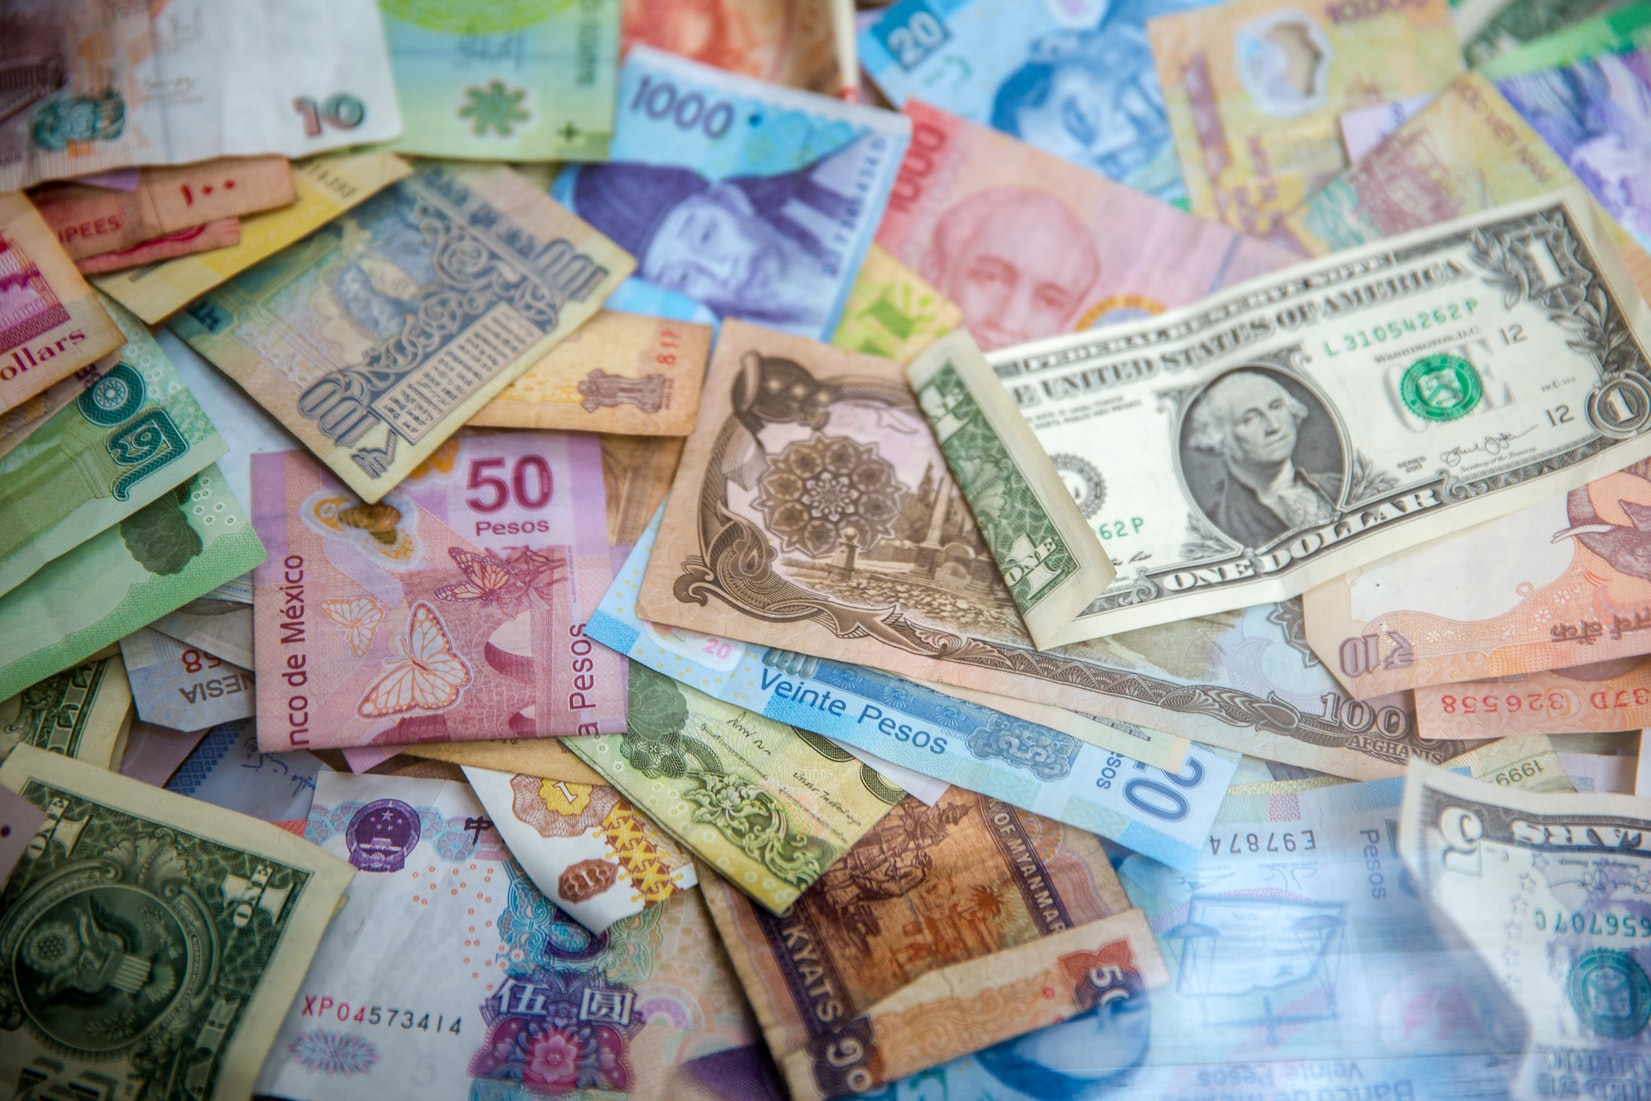
\includegraphics[width=\linewidth]{images/currencies.jpg}			% define cover picture
\end{textblock}


\color{black}

% Institution / titel / subtitel / authors / experts:
%---------------------------------------------------------------------------
\begin{flushleft}

\vspace*{115mm}

\fontsize{24pt}{26pt}\selectfont 
\heading				\\							% Read heading from file leader/title.tex
\vspace{2mm}

\fontsize{14pt}{18pt}\selectfont\vspace{0.3em}
Applied Data Science in an Industrial Banknote Image Recognition Framework			\\				% Insert subheading
\vspace{5mm}


% Abstract (eingeben):
%---------------------------------------------------------------------------


\begin{textblock}{150}(28,225)
\fontsize{10pt}{17pt}\selectfont
\begin{tabbing}
xxxxxxxxxxxxxxx\=xxxxxxxxxxxxxxxxxxxxxxxxxxxxxxxxxxxxxxxxxxxxxxx \kill
Degree course:	\> [BSc Informatik]	\\		% insert name of degree course
Authors:		\> [Sophie Haug]		\\					% insert names
Constituent:	\> [CI Tech Sensors AG]					\\							% insert names
Experts:		\> [Prof. Dr. Macha Kurpicz-Briki]				\\							% insert names
Date:			\> \versiondate					\\							% read from file leader/version.tex
\end{tabbing}

\end{textblock}
\end{flushleft}

\begin{textblock}{150}(28,280)
\noindent 
\color{bfhgrey}\fontsize{9pt}{10pt}\selectfont
Berner Fachhochschule | Haute \'ecole sp\'ecialis\'ee bernoise | Bern University of Applied Sciences
\color{black}\selectfont
\end{textblock}


\end{titlepage}

%
% ===========================================================================
% EOF
%
		% activate for frontpage with picture
% Control of versions :
% -----------------------------------------------

\begin{textblock}{180}(15,150)
\color{black}
\begin{huge}
Versions
\end{huge}
\vspace{10mm}

\fontsize{10pt}{18pt}\selectfont
\begin{tabbing}
xxxxxxxxxxx\=xxxxxxxxxxxxxxx\=xxxxxxxxxxxxxx\=xxxxxxxxxxxxxxxxxxxxxxxxxxxxxxxxxxxxxxxxxxxxxxx \kill
Version	\> Date	\> Status			\> Remarks		\\
0.1	\> 01.08.2013	\> Draft		\> Lorem ipsum dolor sit amet	\\	
0.2	\> 21.08.2013	\> Draft		\> Phasellus scelerisque	\\ 
0.3	\> 02.09.2013	\> Draft		\> Donec eget aliquam urna. Lorem ipsum dolor sit amet	\\ 
1.0	\> 26.01.2014	\> Final		\> Lorem ipsum dolor sit ametPhasellus scelerisque, leo sed iaculis ornare 	\\ 
1.1	\> 31.01.2014	\> Correction	\> Layout changed	\\
1.2	\> 07.02.2014	\> Addition		\> Chapter 1.1 extended	\\
\end{tabbing}

\end{textblock}

\cleardoubleemptypage
\setcounter{page}{1}
\cleardoublepage
\phantomsection 
\addcontentsline{toc}{chapter}{Management Summary}
\chapter*{Abstract}
\label{chap:abstract}

In this project concepts and methods for collecting and preparing data for Currency Adaption are presented, in the context of the company CI Tech Sensors in Burgdorf.
The currency data needed to train and develop algorithms in CI Tech's currency recognition and classification framework should be provided as centralized labelled data sets. These data sets should be generated automatically from the centralized Data Lake. This project proposes a new data container ``NoteSet``, as well as exemplary workflows to achieve this goal.
The implementation was done in Python and using the Jupyter Notebook environment.
\cleardoubleemptypage
%---------------------------------------------------------------------------

% Table of contents
%---------------------------------------------------------------------------
\tableofcontents
\cleardoublepage
%---------------------------------------------------------------------------

% Main part:
%---------------------------------------------------------------------------
\pagenumbering{arabic}

\chapter{Introduction}
\label{chap:projectintroduction}

\section{Introduction}
\label{sec:introduction}

\subsection{Purpose of this document}
\label{sec:purpose}
This document serves as a documentation for the project ``Data Collection and Preparation for Currency Adaptation``which is carried out in the scope of the BFH module ``Project 2``  BTI7302. \par
The client of the project is the company CI Tech Sensors AG (subsequently referred to as CI Tech) and the project is supervised on the part of CI Tech by Lukas Burger, head of application software.

The project is supervised on the part of BFH by Prof. Mascha Kurpicz-Briki.

\subsection{Vision}
In the scope of this project a process for the data collection and preparation for the currency adaptation workflow should be developed.
Namely, the currency data needed to train and develop algorithms in CI Tech's currency recognition and classification framework should be provided as centralized labelled data sets. These data sets can be generated automatically from the centralized Data Pool, they are version controlled and a uniform process for their updating and management will be implemented.
With this change, it will be possible to directly track the influence a new banknote recording has on an existing currency recognition software. Also it will be possible to use dedicated sub-data sets for training specific algorithms, for example data sets consisting of banknotes with a dogear.
\chapter{Project Goals}
\label{chap:projectgoals}

\section{Initial Position}
\subsection{Background}
The 80/20 rule of Data Science states that most data scientist spend about 20\% of their time on actual data analysis and 80\% of their time finding, cleaning and preparing data. The process of readying data for the training, testing and implementation of an algorithm thus is not only a highly important step in the Data Science Lifecycle, it's maybe the costliest.\par
CI Tech Sensors has over 30 years experience in the field of Banknote Image recognition. One of its core competences is the development of currency adaptation software. Namely the so-called Currency Data File is a software, which is loaded onto the banknote reader, and enables it to identify and classify banknotes for specific currencies, as well as determine their fitness and authenticity. This software is continuously updated and developed by a dedicated team of Currency Adaptation Specialists at CI Tech Sensors, whose work relies on the availability of a huge data pool of Banknote Raw Data. \par
Over the last three years, there has been ground-breaking shift in raw data management: From folder-based data storage on both local and central file drives -  which heavily relied on filenames for identification and was thus prone to ambiguity and duplication of data - towards a centralized data pool, where each file was given a unique ID. At the same time a cloud based Microservice architecture (MOVEm Data Management Toolchain) for the management and maintenance of this data pool was developed.
This development comes with a number of exciting possibilities, some of which to explore is the goal of this project. The focus will be on the collection and preparation of tailored banknote sets.\par

In earlier days, the collection and preparation of banknote data had to be manually done by the Currency Adaptation Specialist. They would have to navigate to the relevant folder, select the relevant files and sort them by denomination, emission, orientation and other criteria, an information taken from a file's annotation. Not only is this process cumbersome and error-prone in itself, it also solely relies on the file annotation, which is made by a human annotator before the actual banknote recording, and thus can contain errors as well. \par
Today it's already possible to group banknote raw data into sets, using a text-based file format called notelist file . Adaptations specialists will manage and create their own notelist files locally according to their specific needs. Notelists contain references to individual file IDs and Note IDs as well as additional annotational information and the file path where files can be found. However this format comes with some problems of its own.\par

\subsection{Overview of the existing CI Tech adaptation toolchain }

In this section a short overview is given over some of the tool in the existing CI Tech adaptation toolchain. This list is by far not exhaustive and only names the tools which are mot relevant to the project at hand
\begin{itemize}
\item \emph{MCM} (MOVE Currency Data Modeller) is a desktop application and the main tool of currency adaptation specialists in their daily work. It is used to develop, test and adapt so called \emph{Currency Data Files}, the software which is loaded onto the banknote reader and enables it to recognize and classify banknotes. MCM is a software monolith that has grown and extended its functionality over decades, but it doesn't lend itself very easily to modularization. MCM is also the interface to the entire algorithmic framework. Recordings of banknotes can be loaded from the filesystem as .NIF files (binary files) or .nl (XML Format) files. The latter also allows loading notes from the central Data Pool via MFX instead of the local file system.

\item \emph{MFX} (MOVE File Index) is a web based microservice that allows the lookup of files from the central Data Pool. Namely, it allows to retrieve the storage path in the pool for a given File ID. Using this service, MCM can load files by File ID instead of a file path.

\item \emph{MDS} (MOVE Data Service) is a web based microservice that allows the lookup of note and image data. It allows to query the most relevant note data found in the (binary) .NIF files as well as images via REST api. A future vision which is in ongoing development is that entire sets of notes could be loaded into MCM via this REST interface instead of parsing large amounts of binary data. 


\end{itemize}
\subsection{Stakeholders}
\begin{itemize}
\item The Head of Application Software will supervise the project and provide technical advice
\item The Head of Currency Adaptation will provide additional support from the perspective of Currency Adaptation specialists.
\item The Currency Adaptation team will be the primary user group
\end{itemize}

\section{Project Goals}
\label{sec:goals}


\subsection{Accurate, consistent and complete reference data sets}
The goal is to have accurate and consistent data sets, which are generated and persisted in a way that makes use of the Microservice based MOVEm Data Management Toolchain. Namely these test sets should fulfil the following criteria:

\begin{itemize}
\item Accuracy: Data in test sets has been checked for correct labeling and or given a label in case it was missing.
\item Consistency: Different adaptations for the same currency should use the same data sets. 
\item Completeness: In the generation of reference note data sets, all data in the pool should be considered.

\end{itemize}




\subsection{Mechanism for subclassifying Data Sets according to context-dependent criteria}

It should be possible to generate data sets according to user specific criteria like: "All EUR notes that were classified as fake", "All USD notes for which tape was detected". 
A process should be installed which allows specialist users to generate such datasets from queries. These datasets will have to fulfil the same criteria as the reference data sets.

\subsection{Automated process for generating and maintaining Reference Note Data Sets}

A process has to be defined for generating Reference Data Sets automatically as well as updating and expanding them when new data is added to the Data Pool. A process has to be defined for generating Reference Data Sets automatically as well as updating them when new data is added to the Data Pool. Part of this process is also the management of Reference Data Sets in a Version Control System. 

\subsection{Technical Analysis of the existing Toolchain}

To achieve the previously listed goals, the introduction of a new data container will be necessary to make the existing toolchain compatible with this new paradigm. While this shift can only happen over a longer period, it would be very undesirable to have a new data container or format which will only be deployable for a part of the toolchain. The goal is therefore to have an assessment on the feasibility of implementing the new data container into the existing toolchain. 


\subsection{Introduction of Data Science Workflows in the company}
Another less technical goal, is to familiarize users with certain Data Science workflows. This entails showing by presenting this project how the existing microservice can be used to gain knowledge about note data and generate data sets, as well as familiarize expert users (who might want to use similar workflows to generate their own data sets) with the Jupyter Notebook framework.
\chapter{Project Methods}
\label{chap:projectsteps}


\section{Introduce Note Sets as a new note data container}
\label{noteset_goal}
We will introduce Note Sets as a new data container for referencing and persisting sets of note data. While these Note Sets will be exported to files, they do not constitute a file format in the narrower sense, but rather a new paradigm as how to think of collection of notes: No longer as notes that were recorded in the same transaction and thus in the same binary file (in earlier times this was the only way one could think of collections of notes), but as a collection of IDs.

The note set data container will have the following advantages:
\begin{itemize}
\item Compactness: Note Sets will be minimalist in the sense that notes are references by ID only. There is no additional information like annotation stored in the note set format.
\item Independency of file locations: With the introduction of MFX the actual location of a file in the pool becomes redundant. Therefore, the note set does not store any file paths.
\item Equivalence with respect to annotation: Unlike the Notelist format, Note Sets will no longer have an individual annotation per note. Rather, they have at most one annotation per note set, which is to be persisted in the note set's filename. Thus, note sets are considered equivalent with respect to annotation
\end{itemize}
Meanwhile, the new data container must at least satisfy the following requirements:
\begin{itemize}
\item Convertability to and from the existing Notelist format. The Notelist format has been established as the standard way of storing data sets in Currency Adaptation. Even if one were to pursue the goal of replacing the Notelist format by the Noteset format, convertability would be needed at least for a period of transition. The reasons for that are that a) Noteset import is supported by MCM however in a yet limited way. b) the Python MCM wrapper library mcmp, which is used to load notes and run algorithms from outside MCM, does currently not support the loading of Notesets.
 \item Differentiability. Since they are so minimalist, Note Sets are more ideal than previous formats for quick comparison. We need a way to compare and find the difference between Note Sets reliably and efficiently.
\end{itemize}

The Note Set data container is introduced in a small python library providing the abovementioned functionality. This library is deployed as a python package and can be used in the python toolchain, including MDS and MFX, as well as in Jupyter notebooks. In a later step it remains to analyze the feasibility of introducing this data container in the .NET toolchain as well.

\section{Implement Processes for Automated NoteSet Generation}
Using different methods and for a set of exemplary currencies a first version of NoteSets are generated from the Data Pool, In the course of this existing client software of MDS and MFX are extended to allow for more complex queries.\par
In a first phase Jupyter Notebooks are used to generate the NoteSets. Different methods and their results, i.e. the resulting NoteSets, will be compared and presented to the Currency Adaptation Team. Once the NoteSet generation process has been refined on a technical level, it remains to decide how to include it in the adaptation specialist's workflow.\par
The NoteSet generation workflow in this development phase can be described as follows: 
\begin{enumerate}
\item Crawl MFX for a chosen currency to obtain all file paths of .NIF files for that currency
\item With a list of all FileIDs and corresponding filepaths, use a labeling method to label all the notes in alle the files
\item Based on the obtained labeling, split the set of all Notes into labelled NoteSets (within a NoteSet, all elements have the same label)
\end{enumerate}
It remains thus to choose a labeling methods. I extracted the following four methods which can be outlined as follows:
\begin{enumerate}
\item For each note in the set of all notes, query MDS to obtain the recognition and classification done by the reader for this note. We use the banknote reader (and the CDF which was loaded at the time of recording) as the labeller. This is the most straightforward way, since all that is done is query existing information from the MDS REST API. No new information is generated.
\item Use the MOVEmSimulator to simulate the reader on the chosen set of notes and a chosen .CDF. Use the information found in the .NIFs generated by the Simulator to group and label the Note Sets. This method is more complicated and time consuming than the first one, but it's also more generic, because it makes us independent from the .CDF which was used in the original recording. For example, the original .CDF used in the actual recording might classify a note as Category 3 (suspected counterfeit), but might now be outdated since the lates .CDF for the same currency classifies the same note as Category 2 (proven counterfeit). On MDS, the information generated in the original recording is stored, therefore, this note will always be a Category 3 note if we use the first method. If we let the simulator process the chosen set of .NIF files first, using the latest CDF, we will get the most up to date information, namely the results a physical reader would calculate using the most recently released .CDF.
\item Load all the notes from the set of all notes into MCM and use algorithm(s) from the algorithmic framework of MCM to determine properties of each note based on which the notes can be labelled. We use MCM as the labeller. To do this in an automated way, a Python wrapper for MCM has to be used, which unfortunately only allows restricted use of MCM.
\item Use an algorithm external to MCM as a kind of plug-in to process and label the notes. This is the most experimental method, but maybe also the most interesting one. It has the advantage that we are free of MCMs monolithic architecture in our labeling process, but also the challenge that the MCM algorithmic framework is highly developed and refined and can hardly be bested by an external classifier.
\end{enumerate}
\par Figure \ref{fig:ns_mds} to \ref{fig:ns_plugin} visualize these different approaches.

\begin{figure}[!htb]
\minipage{0.49\textwidth}
  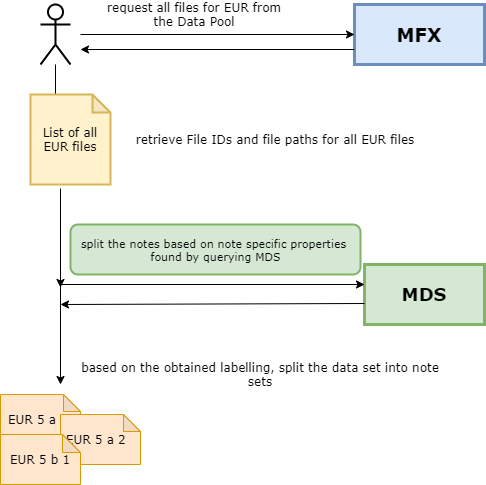
\includegraphics[width=\linewidth]{images/label_mds_approach.png}
  \caption{NoteSet Generation with MDS labeling}\label{fig:ns_mds}
\endminipage\hfill
\minipage{0.49\textwidth}
  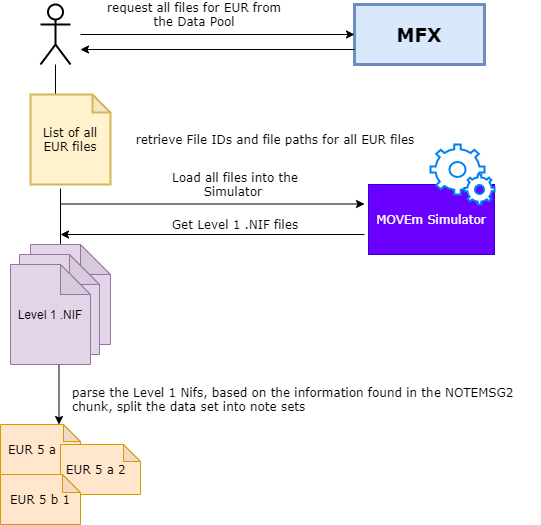
\includegraphics[width=\linewidth]{images/label_simulator_approach.png}
  \caption{NoteSet Generation with MOVEm Simulator labeling}\label{fig:ns_sim}
\endminipage\hfill
\minipage{0.49\textwidth}
  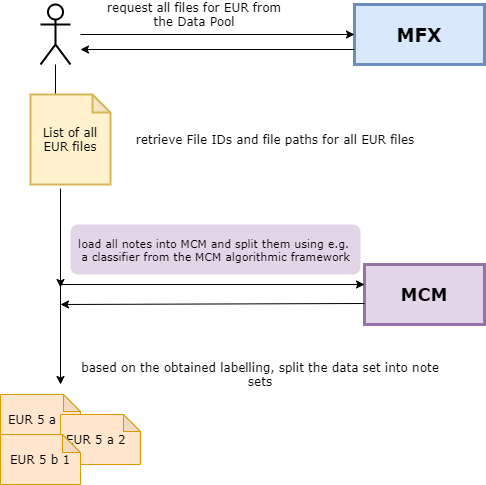
\includegraphics[width=\linewidth]{images/label_mcm_approach.png}
  \caption{NoteSet Generation with MCM labeling}\label{fig:ns_mcm}
\endminipage\hfill
\minipage{0.49\textwidth}%
  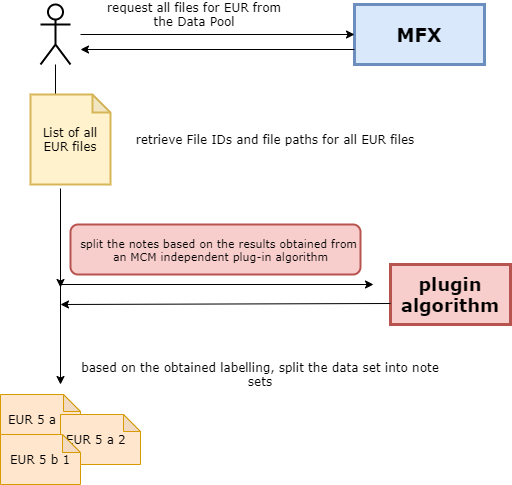
\includegraphics[width=\linewidth]{images/label_plugin_approach.png}
  \caption{NoteSetGeneration with Plugin Algorithm}\label{fig:ns_plugin}
\endminipage
\end{figure}

In the course of implementing the project the focus shifted almost entirely on the method of labeling via MDS and the MOVEm Simulator. In a first stage I tried to use MCM as a labeller, but discarded this mainly because of performance reasons. MCM is already a very resource-intensive piece of software and accessing it via a Python wrapper from Jupyter had another negative impact on the performance. In addition, the python wrapper for MCM is quite limited as only a number of MCM functions are accessible and MCM is impossible to debug when accessed via Python. \par
The usage of a plugin algorithm is still a promising option especially if one would like to challenge an existing algorithm (e.g. classifier) by comparing its result with a generic image classifier. It turned out however that the users' main need at this point in time is not to gather new knowledge from the existing data but rather to just find ways of generating useful datasets. Given that the need of introducing a new algorithm was less urgent. 

\section{Introduce NoteSet loading in MCM}
Since MCM already uses MFX, it is able to load NIF files by File ID only, thus nothing stands in the way of loading Notes by ID, i.e. as a set of Note IDs. Therefore a feature is added in MCM which allows loading and exporting of NoteSets. This should be done with as little cost as possible as introducing bigger changes and new models into MCM is always very complex and delicate. The idea is to allow passing NoteSets in the MCM View layer, but converting them into standard MCM Notelist objects before they are passed to deeper layers. 

\chapter{ NoteSet Data Container Specification}
\label{chap:technicaldocu}

\section{NoteSet Specification}
\subsection{Motivation}
By introducing the NoteSet as a new data container the primary goal is not to introduce a new data format. Firstly, because this would entail a longer process of defining a format schema and approval of various departments, the potential users of the new format, as well as a long introduction phase. Secondly, a data format is always restrictive in that it imposes an absolute way of how data should be thought of. The goal of introducing the NoteSet is exactly the opposite: We want users to think of a data collection as exactly that and not more: A collection of data elements, that at least for now does not come with a set of restrictions and rules of its own, or with as little as possible. In our case, this means that a NoteSet is just a set of notes which can be found in our Data Lake, or put differently: a set of Note IDs. In section \ref{noteset_goal} we listed the advantages and requirements for the new data container. In this section the steps undertaken to reach them will be specified.
\subsection{Problems with the Notelist format}
Even though the Notelist format (see section \ref{section:notelist}) has been established as a de facto standard, there are some disadvantages that come with it and that the introduction of the NoteSet data container hopes to address:
\begin{itemize}
\item Too much flexibility: Since Notelists are annotatable on a per-note basis and not on a per-set basis, there is no limit to mixing notes from different currencies, denomination etc. within the same list. This can lead to the temptation to store all notes a user works with over a timespan of months or longer in one single big Notelist. However this defeats one of the Notelist's original purposes namely creating more clarity by storing notes into use-case-specific sets that can be re-used by others. 
\item Readabililty: Large notelists can get hard to read (and even harder to compare), due to the bulk of annotational information which in most cases is redundant. 
\item Insufficient congruity with MOVEm Data Service APIs: Since the Notelist Format requires the presence of a file path, it is not possible to directly generate Notelists from MDS queries. If we query notes from MDS we get back a JSON structure containing the note data stored in the NIF, but no file location (The NIF does not store file location). Thus, we have to get the file path for each File ID with an additional MFX query and consequently increase the amount of queries. This is still feasible, but it slows down the generation of data sets.\footnote{The necessity of the file path in the Notelist hails from a time where the MFX service had not yet been establised. Therefore the Notelist needed to know the file location of each NIF on the local file system, in order to be able to load it. Today, where MFX is used to load the notes from the Data Lake, the NIF's File ID is enough information for locating and loading it.}\par Furthermore, the Notelist format requires the presence of an outdated GUID for each note. In other words, while the Note ID is the unique note identifier in the universe of MDS and MFX, the Notelist always requires an additional identifier.
\end{itemize}
\subsection{NoteSets as equivalence classes}
One distinguishing feature of NotSets is that they will not have a per-note labelling but one labelling for the entire set, the NoteSet annotation. This is in the spirit of the adaptation specialist's way of working with data, insofar that they are generally not interested in the individual notes as such, but rather in an algorithm's performance on a particular set of -- correctly labelled -- notes. Thus we can think of NoteSets as equivalence classes where the equivalence relation is defined by the NoteSet's annotation. The NoteSet Annotation is specified below in section \nameref{ns_annotation_spec}
\subsection{Serialization}
\label{subsection:ns_serialization}
Since NoteSets are basically just a collection of IDs, we will store them as text files in ASCII format. In a generic NoteSet, each line will represent a note. We do allow the following rules and elisions, some of whose usage will make the serialized form more compact, if parsing slightly more complicated:
\begin{enumerate}
\item Notes within the same file can be listed on the same line, e.g.:
\begin{align*}
374DB8C13B9B1DB8C42C1B109DE3BBD5:1 \\
374DB8C13B9B1DB8C42C1B109DE3BBD5:2 \\
374DB8C13B9B1DB8C42C1B109DE3BBD5:3 \\
374DB8C13B9B1DB8C42C1B109DE3BBD5:4 \\
374DB8C13B9B1DB8C42C1B109DE3BBD5:5 \\
374DB8C13B9B1DB8C42C1B109DE3BBD5:12
\end{align*}
is equivalent to:
\begin{align*}
374DB8C13B9B1DB8C42C1B109DE3BBD5:1-5,12
\end{align*}
\item If we mean to include all the notes in a file, we can reference them just be the File ID. Thus, assuming that a file contains 100 note recordings:
\begin{align*}
374DB8C13B9B1DB8C42C1B109DE3BBD5
\end{align*}
is equivalent to:
\begin{align*}
374DB8C13B9B1DB8C42C1B109DE3BBD5:1-100
\end{align*}
and also equivalent to:
\begin{align*}
374DB8C13B9B1DB8C42C1B109DE3BBD5:1 \\
374DB8C13B9B1DB8C42C1B109DE3BBD5:2 \\
374DB8C13B9B1DB8C42C1B109DE3BBD5:3 \\
374DB8C13B9B1DB8C42C1B109DE3BBD5:4 \\
...\\
374DB8C13B9B1DB8C42C1B109DE3BBD5:100
\end{align*}
\item We will allow comments, preceded by \#
\item Any software with a NoteSet export feature will use the generic way of just listing the individual Note IDs and not use the abbreviated forms presented above
\end{enumerate}
\begin{figure}[!htb]
\minipage{0.49\textwidth}
  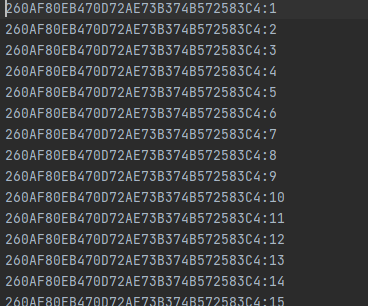
\includegraphics[width=\linewidth]{images/notesetpicture1sm.png}
  \caption{Extract of a generic NoteSet file}\label{fig:ns_example_1}
\endminipage\hfill
\minipage{0.49\textwidth}
  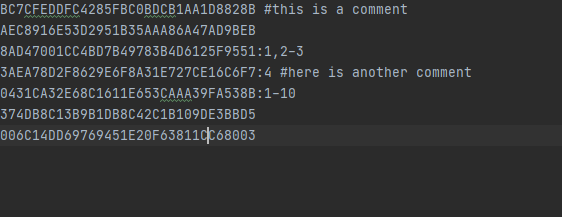
\includegraphics[width=\linewidth]{images/notesetpicture2.png}
  \caption{Extract of a NoteSet file using abbreviations and comments}\label{fig:ns_example_2}
\endminipage\hfill
\end{figure}

\subsection{The pynoteset library}
Since there is already a comprehensive Python toolchain for Adaptation Software, it was an obvious choice to implement a library  \emph{pynoteset}-  This small library can generate NoteSet object from ASCII-files or lists of FileIds/NoteIds, and perform the classical set-theory operations on NoteSets. The features of the pynoteset library can be summarized as follows: 
\begin{enumerate}
\item generate NoteSet objects from files
\item export NoteSet objects to ASCII files
\item annotate NoteSet objects and parse string annotations
\item merge NoteSet objects: for two NoteSets $A$ and $B$ generate the NoteSet $A \cup B$.
\item intersect NoteSet objects: for two NoteSets $A$ and $B$ generate the NoteSet $A \cap B$.
\item compare NoteSet objects: for two NoteSets $A$ and $B$ generate the NoteSet $A\backslash B$ and $B\backslash A$. 
\end{enumerate}

The library consists of three main classes, the NoteSet class, the NoteSetAnnotation class and the NoteSetConverter class. The latter's purpose is to generate NoteSet objects from files and lists of strings, a functionality that was outsourced into a converter class because of a dependency on MDS, which I didn't want to have in the NoteSet class itself\footnote{The reason for this dependency is the generosity of the NoteSet serialization syntax as specified in section \ref{subsection:ns_serialization}: Remember that if we mean to include all the notes in a file, we can reference them just be the File ID. Internally however, the NoteSet object has to know the number of notes in a file. Therefore, in the case where just a File ID is given, we have to query the number of notes (property ``note\_count``) from the MDS API.} See the pynoteset class diagram figure \ref{fig:pynoteset} for reference.\
Furthermore, a converter class NoteSet2Notelistfile has been added to the library \emph{notelistfile}, which allows the conversion of NoteSets to Notelist, the standard XML based format currently in use (cf. section \ref{section:notelist}). This functionality is particularly powerful since a majority of the Python toolchain already uses a Notelist class internally. The converter thus provides an interface for the NoteSet object to be used in other tools.\par
For deployment of this library a Bitbucket CI/CD pipeline is used, which deploys the package to a software repository manager (JFrog Artifactory). Thus registerered Artifactory users can install the pynoteset package like any other using e.g. \emph{pip}.
\begin{figure}
 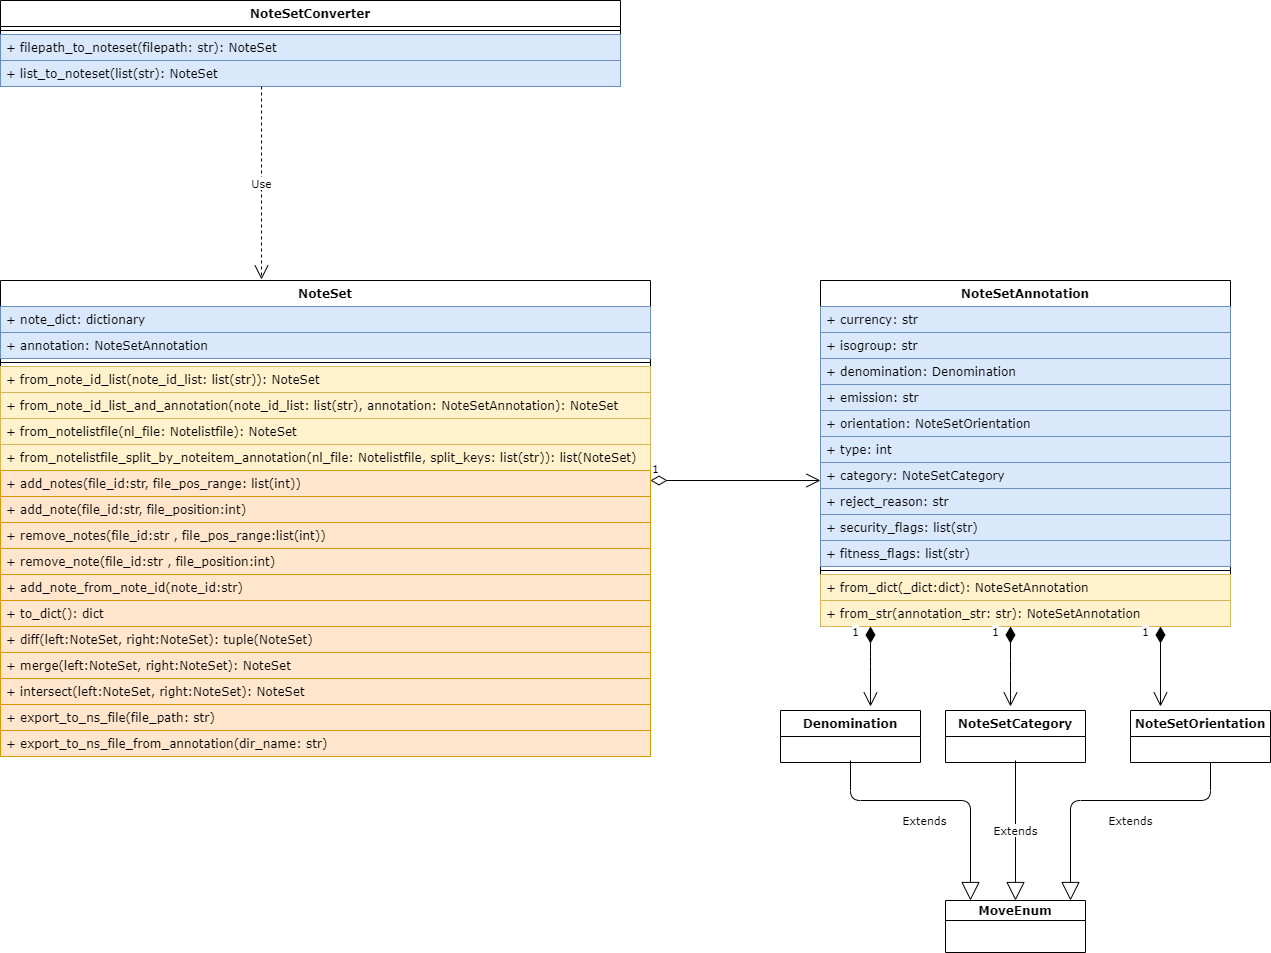
\includegraphics[width=\linewidth]{images/pynoteset.png}
   \caption{Class Diagram of \emph{pynoteset}}\label{fig:pynoteset}
\end{figure}

\section{NoteSet Annotation Specification}
\label{ns_annotation_spec}

\subsection{Motivation}
As already mentioned, we introduce NoteSets as a container for notes which are equivalent with respect to a yet to be defined annotation, the labeling of the set. Since the NoteSet itself is basically just a set of IDs or keys, all other substantial information will be in the annotation. The first challenge is to select the properties which should be part of the annotation. The second is the question of how to persist the annotation within the NoteSet. Since we do not want to introduce a new format definition, it's not possible to add the annotation as a sort of header in an XML or JSON format. This would mean that a new format has been introduced and some kind of schema would have to be defined for it. \par
The only option that remains is thus to store the set's annotation within the filename itself when exporting a NoteSet. For this a special file format string has to be introduced (see below).
\subsection{Criteria for selecting annotational elements}
The selection of the elements which should be part of the annotation was overall not that easy, on the one hand because there are hundreds of properties in a NIF file and we want to be as specific as possible, on the other hand, a NoteSet's annotation should be as simple as possible, namely because we want to persist the annotation in the filename, which ideally should be a readable and not too long string.
Finally after having consulted with the adaptation specialist team, the selection was done by the following criteria: The mandatory properties are properties which are needed to identify a particulat type of note in MCM. The optional properties (with the exception of comment) are criteria for which are not mandatory to identify a note, but for which it is likely that a user wants to split or filter a set of notes by them when analyzing or training algorithms.
\subsection{Mandatory Elements of the NoteSet Annotation}
The following attributes form the mandatory part of the NoteSet's annotation. These are all derived from properties set in the NOTEMSG2 chunk of the NIF file. 
\begin{description}
  \item[Currency] Corresponds to the ISO string matching the the numeric ISOCODE value in the NOTEMSG2 Chunk.
  \item[IsoGroup] A sub-specification of a currency that is mainly used for the currency GBP (Great Britain Pound), which has different banknotes and issuers for the groups England (BOE), Scotland (SCO), Northern Ireland (IRL), Guernsey (GUE), Jersey (JER) and Isle of Man (MAN). For example, the England GBP would be abbreviated as GBPBOE, the Irish one as GBPIRL.
  \item[Emission] Emission of the notes in the NoteSet, corresponds to the value of the Chunk EMISSION in NOTEMSG2
  \item[Orientation] Orientation of the notes in the NoteSet, corresponds to to ORIENTATION in NOTEMSG2
\item[Type] NoteType, a numeric value to identify the CDF reference note this note is matched to. In some cases there is more than one reference note for the same denomination, emission and orientation (for example when a currency has different issuers/printers that each print their own distinctive banknotes)
\end{description}

\subsection{Optional Elements of the NoteSet Annotation}
The following attributes are optional elements of a NoteSet Annotation. They are not identifying properties but allow to specify a NoteSet.

\begin{description}
\item[Class] Corresponds to the value CATEGORY in NOTEMSG2 Chunk and is an attribute for authenticity and fitness of a banknote, for example, Category 4a notes are authentic and fit notes, Category 2 are counterfeits. It's a likely use case that a user would want to split notes across a currency by category to train and analyze fitness and security algorithms. 
\item[Security and Fitness flags Flags] Security and Fitness Flags are set by certain algorithms and indicate that a note might be classified as unfit or counterfeit. For example, the fitness flag STAIN indicates that the note has some kind of smudging, the security flag ROBBERY\_INK indicates that the presence of robbery ink was detected. 
\item[Reject Reason] This is an enum value found corresponding to the value REJECT\_REASON in NOTEMSG2 chunk. It indicates the reason why a note was rejected or that it was not rejected.
\item [Comment] This is an optional comment added by the user and the only value within the NoteSet annotation which does not come from the NIF file
\end{description}

\subsection{Specifying the file format string}
As already stated, the NoteSet's annotation is to be converted into a filename when exporting a NoteSet to ASCII. The file format string to be constructed has to be readable, complete and indicate the optionality of properties, i.e. distinguish the optional properties from the mandatory ones. Finally, the goal is to codify the format into a regular expression and implement an annotation parser in the python noteset library \emph{pynoteset}.
\subsubsection{Preliminary Decisions}
\begin{itemize}
\item The file format string must be defined in a regular expression. Thus any tool which would later adopt the paradigm of NotSets could easily validate NoteSet annotations independent of the programming language.
\item Generic placeholder for non-specified mandatory properties: Since we allow NoteSets to be merged, we have to anticipate the scenario where e.g. a NoteSet contains notes of various denominations. Therefore we need a placeholder for all mandatory properties indicating the state of 'Undefined' or mixed. This placeholder is 'XXX' for currencies and isogroups and 'X' otherwise, a practice which is already in use in the recording of note data and thus one that users are already familiar with. 
\item Allowing of both upper- and lowercase spelling: While it is common to use uppercase notation for currency ISO codes and isogroups and lowercase spelling for emissions, we will allow both upper- and lowercase notation to make the already fairly complicated string format less restrictive.
\end{itemize}
Finally, from these requirements such a regular expression could be defined as follows:

\begin{center} 
\begin{verbatim}
([A-Z]{3}){1,2}_(([0-9]*[.])?[0-9]|X)*_([a-z]|X)_([1-4]|X)_([1-9]+|X)(_CL[1-4])?(_SF\(([A-Z_0-9]+)(&[A-Z_0-9]+)*\))?(_FF\(([A-Z_0-9]+)(&[A-Z_0-9]+)*\))?(_[a-zA-Z0-9]*)?
\end{verbatim}
\end{center} 
The examples in figure \nameref{fig:ns_example} illustrate the application of this regular expression, i.e. some valid NoteSet Annotation file strings
\begin{figure}[!htb]
  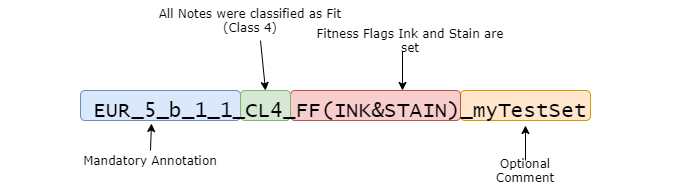
\includegraphics[width=0.49\linewidth]{images/annotation_example1.png}
  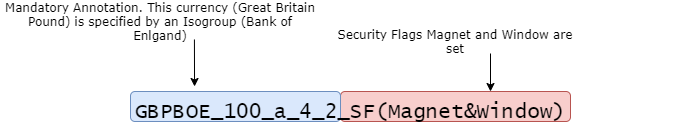
\includegraphics[width=0.49\linewidth]{images/annotation_example2.png}
  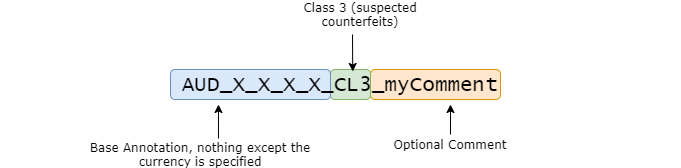
\includegraphics[width=0.49\linewidth]{images/annotation_example3.png}
  \caption{NoteSet Annotation Examples}\label{fig:ns_example}
\end{figure}

A parser for annotation strings was included in the pynoteset library and since we have defined a regex for it, it would be relatively easy to implement this feature in other tools as well.

\section{Integrating the NoteSet Data Container in MCM}
In order to enable MCM to load NoteSets, a minimal viewer was added to one of the main viewers, which allows to copy-paste and load NoteSets, following the syntax specification described in section \ref{subsection:ns_serialization}. Internally, during loading these NoteSets were converted into Notelists, the standard Note data container object used in MCM, thus there was no major MCM refactoring to be done in the course of implementing this feature. Albeit very simple, this viewer was positively received by developers and adaptation specialists likewise. Later on I added a small feature allowing to export MCM Notelists as NoteSets (ASCII files).
\begin{figure}
 \includegraphics[width=\linewidth]{images/mcm_ns_Loader.png}
   \caption{NoteSet Loading Viewer in MCM}\label{fig:ns_loader}
\end{figure}
%---------------------------------------------------------------------------

% Declaration of Authorship
%---------------------------------------------------------------------------
%\cleardoublepage
%\phantomsection 
%\addcontentsline{toc}{chapter}{Declaration of authorship}
%\chapter*{Declaration of primary authorship}
\label{chap:declaration_authorship}

\vspace*{10mm} 

I / We hereby confirm that I / we have written this thesis independently and without using other sources and resources than those specified in the bibliography. All text passages which were not written by me are marked as quotations and provided with the exact indication of its origin. 

\vspace{15mm}

\begin{tabbing}
xxxxxxxxxxxxxxxxxxxxxxxxxxxxxx\=xxxxxxxxxxxxxxxxxxxxxxxxxxxxxx\=xxxxxxxxxxxxxxxxxxxxxxxxxxxxxx\kill
Place, Date:		\> [Biel/Burgdorf], \versiondate \\ \\ 
Last Name/s, First Name/s:	\> [Test Peter] 	\> [M\"uster R\"os\"a] \\ \\ \\ \\ 
Signature/s:	\> ......................................\> ...................................... \\
\end{tabbing}

%---------------------------------------------------------------------------

% Glossary
%---------------------------------------------------------------------------
\cleardoublepage
\phantomsection 
\addcontentsline{toc}{chapter}{Glossay}
\renewcommand{\glossaryname}{Glossay}
\printglossary
%---------------------------------------------------------------------------

% Bibliography
%---------------------------------------------------------------------------
\cleardoublepage
\phantomsection 
\addcontentsline{toc}{chapter}{Bibliography}
\bibliographystyle{IEEEtranS}
\bibliography{database/bibliography}{}
%---------------------------------------------------------------------------

% Listings
%---------------------------------------------------------------------------
\cleardoublepage
\phantomsection 
\addcontentsline{toc}{chapter}{List of figures}
\listoffigures
\cleardoublepage
\phantomsection 
\addcontentsline{toc}{chapter}{List fo tables}
\listoftables
%---------------------------------------------------------------------------

% Index
%---------------------------------------------------------------------------
\cleardoublepage
\phantomsection 
\addcontentsline{toc}{chapter}{Index}
\printindex
%---------------------------------------------------------------------------

% Attachment:
%---------------------------------------------------------------------------
\appendix
\settocdepth{section}
\chapter*{APPENDICES}
\addcontentsline{toc}{chapter}{APPENDICES}

\begingroup\let\clearpage\relax
\chapter{The pynoteset library}
\label{chap:appendix_pns}
\endgroup

The pynoteset library was developed within the scope of this project. Its purpose is to generate and handle the newly introduced NoteSet data container. This small library can theoretically be deployed in the entire Python toolchain of application software at CI Tech. An analogous implementation in C\# for the .NET toolchain is still pending

\section{The NoteSet class}
This is the base class representing a noteset object. A NoteSet represents a set of Note IDs. It can optionally contain an annotation property, which is of type NoteSetAnnotation.
\subsection{from\_note\_id\_list(note\_id\_list)}
\subsubsection{Description}
Generates a NoteSet object from a list of Note IDs
\subsubsection{Parameters}
\begin{description}
\item [note\_id\_list] A list of strings representing Note IDs.

\end{description}

\subsection{from\_note\_id\_list\_and\_annotation(note\_id\_list, annotation)}
\subsubsection{Description}
Generates a NoteSet object from a list of Note IDs and a NoteSetAnnotation object.
\subsubsection{Parameters}
\begin{description}
\item [note\_id\_list] A list of strings representing Note IDs.
\item [annotation] NoteSetAnnotation
\end{description}


\subsection{from\_notelistfile(nl\_file)}
\subsubsection{Description}
Generate a NoteSet object from a Notelistfile object, i.e. convert a Notelistfile into a NoteSet.
\subsubsection{Parameters}
\begin{description}
\item [nl\_file] Notelistfile 
\end{description}

\subsection{diff(noteset\_1, noteset\_2)}
\subsubsection{Description}
Find the difference of two NoteSets. Return two notesets:
\begin{itemize}
	\item NoteSet of all elements contained in noteset\_1 but not noteset\_2
	\item NoteSet of all elements contained in noteset\_2 but not noteset\_1
\end{itemize}
\subsubsection{Parameters}
\begin{description}
\item [noteset\_1] NoteSet
\item [noteset\_2] NoteSet
\end{description} 

\subsection{merge(noteset\_1, noteset\_2)}
\subsubsection{Description}
Merge two NoteSets into a new NoteSet
\subsubsection{Parameters}
\begin{description}
\item [noteset\_1] NoteSet
\item [noteset\_2] NoteSet
\end{description} 

\subsection{export\_to\_ns\_file(filepath)}
\subsubsection{Description}
Save a NoteSet as ASCII file
\subsubsection{Parameters}
\begin{description}
\item [filepath] string or path-like object
\end{description}
\chapter{Additional Appendix}
\label{chap:appendix_B}

\section{Test 1}
To an English person, it will seem like simplified English, as a skeptical Cambridge friend of mine told me what Occidental is. The European languages are members of the same family. Their separate existence is a myth. For science, music, sport, etc, Europe uses the same vocabulary. The languages only differ in their grammar, their pronunciation and their most common words. Everyone realizes why a new common language would be desirable: one could refuse to pay expensive translators. To achieve this, it would be necessary to have uniform grammar, pronunciation and more common words. If several languages coalesce, the grammar of the resulting language is more simple and regular than that of the individual languages. The new common language will be more simple and regular than the existing European languages. 

\subsection{Environment}
It will be as simple as Occidental; in fact, it will be Occidental. To an English person, it will seem like simplified English, as a skeptical Cambridge friend of mine told me what Occidental is. The European languages are members of the same family. Their separate existence is a myth. For science, music, sport, etc, Europe uses the same vocabulary. The languages only differ in their grammar, their pronunciation and their most common words. Everyone realizes why a new common language would be desirable: one could refuse to pay expensive translators. To achieve this, it would be necessary to have uniform grammar, pronunciation and more common words.
\chapter{Content of CD-ROM}
\label{chap:appendix_CDROM}

Content of the enclosed CD-ROM, directory tree, etc.
%---------------------------------------------------------------------------

%---------------------------------------------------------------------------
\end{document}

